\headline{{\textbf{\Large\sffamily Shared Canopy:}}\\
          {\textbf{\large\sffamily Friends of Twickenham Bonsai Club}}}
\label{2025-06-canopy}
\begin{window}[%
    0,r,%
    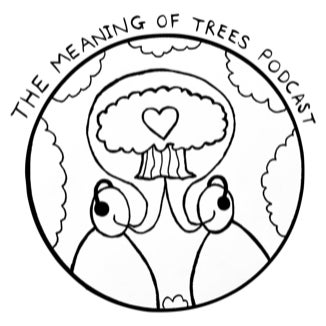
\includegraphics[width=0.45\columnwidth]{2025_06/res/canopy_podcast},%
    %\centerline{\emph{\href{https://linktr.ee/themeaningoftreespodcast}{\emph{The Meaning of Trees Podcast}}.}}%
]  
\noindent
This month, we're thrilled to share a new branch on the bonsai audio tree: \textbf{\href{https://linktr.ee/themeaningoftreespodcast}{\emph{The Meaning of Trees Podcast}}}, hosted by long\--time tree enthusiast and bonsai advocate \textbf{Amelia Williams} (\href{https://www.instagram.com/juglansnigra}{@juglansnigra}).

Amelia has spent over 20 years working with trees---from ancient oaks to tiny junipers---and is currently Director at UK consultancy \href{https://arb.company/amelia-williams/}{The Arb Company}.
A familiar face to many of us at the club (she's given a memorable talk and often visits our shows with her family!), Amelia continues to champion bonsai as both an art and an ecological philosophy.
\end{window}  

In the latest episode, she and co\--host Tom explore the curious, contemplative world of bonsai, and what our relationship with miniature trees might reveal about our care for larger landscapes---and ourselves.
Thoughtful, grounded, and occasionally laugh\--out\--loud funny, it's a perfect listen with a cup of tea, coffee\dots{} or something stronger!

\textbf{\href{https://open.spotify.com/episode/3uEtSKQBxUmvJOnc0TDYbJ?si=OaeP4pslSzmOvNCw2Gw3Lw}{Listen here}} or search \textit{The Meaning of Trees} wherever you get your podcasts.

\vspace{-0.5em}
\begin{center}
    $\cdots$
\end{center}
\vspace{-0.5em}

\noindent
\textit{Got a bonsai\--friendly friend or project worth featuring?}\\
\textit{Share it with us for the next edition of \textit{Shared Canopy!}}
\closearticle
\columnbreak
